% Created 2018-01-09 mar 13:26
% Intended LaTeX compiler: pdflatex
\documentclass[article, a4paper]{memoir}
\usepackage[utf8]{inputenc}
\usepackage[T1]{fontenc}
\usepackage{graphicx}
\usepackage{grffile}
\usepackage{longtable}
\usepackage{wrapfig}
\usepackage{rotating}
\usepackage[normalem]{ulem}
\usepackage{amsmath}
\usepackage{textcomp}
\usepackage{amssymb}
\usepackage{capt-of}
\usepackage{hyperref}
\usepackage{color}
\usepackage{listings}
\usepackage[T1]{fontenc}
\usepackage[utf8]{inputenc}
\usepackage[a4paper]{geometry}
\geometry{verbose,tmargin=2.5cm,bmargin=2.5cm,lmargin=2.5cm,rmargin=2.5cm}
\pagestyle{Ruled}
\usepackage{array}
\usepackage{verbatim}
\usepackage{prettyref}
\usepackage{booktabs}
\usepackage{textcomp}
\usepackage{url}
\usepackage{amsmath}
\usepackage{chemarr}%flechas para reacciones químicas (SFER.tex)
\usepackage{graphicx}
\usepackage{amssymb}
\usepackage{nomencl}
\usepackage[usenames,dvipsnames]{xcolor}

% the following is useful when we have the old nomencl.sty package
% \providecommand{\printnomenclature}{\printglossary}
% \providecommand{\makenomenclature}{\makeglossary}
\makenomenclature

\usepackage[caption=false]{subfig}
%Configuración de los caption
%\PassOptionsToPackage{caption=false}{subfig}%Evita que el paquete subfig lo descabale todo
\captiontitlefont{\itshape}
\captionnamefont{\scshape}
%\captionstyle{\centering}
\hangcaption


\usepackage[spanish]{babel}
\addto\shorthandsspanish{\spanishdeactivate{~<>}}


\usepackage[emulate=units]{siunitx}
\sisetup{per=fraction, fraction=nice, decimalsymbol=comma}
%\usepackage{lscape}
\usepackage{mathpazo}%Letra palatino con fuentes para matemáticas
\usepackage{flafter}%obliga a que los flotantes aparezcan después de su referencia
\usepackage{memhfixc}
\usepackage{mempatch}


\raggedbottom
\sloppybottom
\clubpenalty=10000
\widowpenalty=10000

%\raggedbottomsection
\feetbelowfloat


\usepackage[citestyle=authoryear, backend=bibtex, bibstyle=authoryear, doi=true, url=true]{biblatex}
\addbibresource{../biblio.bib}
\let\cite\parencite

\renewcommand{\bibsection}{%
	\chapter*{\bibname}
	\bibmark
	\phantomsection
	\addcontentsline{toc}{chapter}{\bibname}
	\prebibhook}
% \renewcommand{\bbltechreport}{Informe T\'ecnico}

\usepackage{hyperref}


\hypersetup{
    bookmarks=true,         % show bookmarks bar?
    unicode=true,          % non-Latin characters in Acrobat’s bookmarks
    bookmarksnumbered=false,
    bookmarksopen=false,
    breaklinks=true,
    backref=true,
    pdftoolbar=true,        % show Acrobat’s toolbar?
    pdfmenubar=true,        % show Acrobat’s menu?
    pdffitwindow=false,     % window fit to page when opened
    pdfstartview={FitH},    % fits the width of the page to the window
    pdftitle={Energía Solar Fotovoltaica},    % title
    pdfauthor={Oscar Perpiñán Lamigueiro},     % author
    pdfsubject={Energia Solar Fotovoltaica},   % subject of the document
    pdfcreator={AucTeX/Emacs},   % creator of the document
    pdfproducer={LaTeX}, % producer of the document
    pdfkeywords={radiación solar, energía solar fotovoltaica, energías
    renovables}, % list of keywords
    pdfnewwindow=true,      % links in new window
    pdfborder={0 0 0},
    colorlinks=true,       % false: boxed links; true: colored links
    linkcolor=Brown,          % color of internal links
    citecolor=BrickRed,        % color of links to bibliography
    filecolor=black,      % color of file links
    urlcolor=Blue           % color of external links 
}
	

\DeclareSIUnit\kWh{kWh}
\DeclareSIUnit\Wh{Wh}
\DeclareSIUnit\Wp{Wp}
\DeclareSIUnit\kWp{kWp}
\DeclareSIUnit\amperehour{Ah}
\DeclareSIUnit\celula{celula}

%\spanishdecimal{.} %Para que no lo sustituya automáticamente por comas
\addto\captionsspanish{%
\def\tablename{Tabla}%
\def\listtablename{\'Indice de tablas}}

\renewcommand\nomname{Nomenclatura}
\def\nompreamble{\addcontentsline{toc}{chapter}{\nomname}\markboth{\nomname}{\nomname}}


%\@addtoreset{equation}{section}
%\renewcommand{\theequation}{\thesection.\arabic{equation}}
%\numberwithin{equation}{section}
%\@addtoreset{table}{section}
%\renewcommand{\thetable}{\thesection.\arabic{table}}
%\numberwithin{table}{section}
%\@addtoreset{figure}{section}
%\renewcommand{\thefigure}{\thesection.\arabic{figure}}
%\numberwithin{figure}{section}


%\declarebtxcommands{spanish}{%
 % \def\btxphdthesis#1{\protect\foreignlanguage{spanish}{Tesis Doctoral}}%
%}
%\setbibliographyfont{lastname}{\scshape}%Pone los autores en Small Caps



%Configuración de MEMOIR
%%Pone la fecha en SMALL CAPS y hacia la derecha
%%pagina 60 de memman.pdf
\pretitle{\vfill \begin{flushright} \bfseries \scshape \HUGE \color{BrickRed}}
\posttitle{\par\end{flushright}}

\preauthor{\begin{flushright} \large \scshape}
\postauthor{\par\end{flushright}}

%\date{}
\predate{\vfill \begin{flushright}\large\scshape}
\postdate{\par\end{flushright}\vfill}

\setsecnumdepth{subsection}


% \definecolor{ared}{rgb}{.647,.129,.149}
% \renewcommand{\colorchapnum}{\color{ared}}
% \renewcommand{\colorchaptitle}{\color{ared}}
% \chapterstyle{pedersen}
\chapterstyle{ger}

\setlength{\afterchapskip}{35pt}
\maxtocdepth{section}

%\setcounter{topnumber}{3}
%\setcounter{bottomnumber}{2}
%\setcounter{totalnumber}{4}
\renewcommand{\topfraction}{0.85}
\renewcommand{\bottomfraction}{0.5}
\renewcommand{\textfraction}{0.15}
\renewcommand{\floatpagefraction}{0.7}


%Centra las figuras en los flotantes y los enmarca
\makeatletter
\renewenvironment{figure}[1][]{%
     	\@float{figure}%
		%\begin{framed}    
		\precaption{\rule{\linewidth}{0.4pt}\par}%En las figuras el caption va debajo
		%\hrule\vspace{\onelineskip}
		\centering
		  }{%
		%\end{framed}
		%\postcaption{\rule{\linewidth}{0.4pt}}
		%\vspace{\onelineskip}\hrule
    	\end@float	
}
\makeatother

\makeatletter
\renewenvironment{table}[1][]{%
      	\@float{table}%
		%\begin{framed}    
		\postcaption{\rule{\linewidth}{0.4pt}\par}%En las tablas el caption va encima
		\centering
		  }{%
		%\end{framed}
    	\end@float	
}
\makeatother


\renewcommand{\textfloatsep}{10pt}%Espacio entre el flotante y el texto

%backgroung image
\usepackage{eso-pic} 

%http://stackoverflow.com/questions/240097/how-to-create-a-background-image-on-titlepage-with-latex
\newcommand\BackgroundPic{
  \put(350,-150){
    \parbox[b][0.5\paperheight]{0.5\paperwidth}{%
      \includegraphics[scale=0.5]{../figs/johnny_automatic_old_sun}%
}}}

\newcommand\BackgroundPicLight{
  \put(350,-150){
    \parbox[b][0.5\paperheight]{0.5\paperwidth}{%
 %     \vfill 
%\centering
      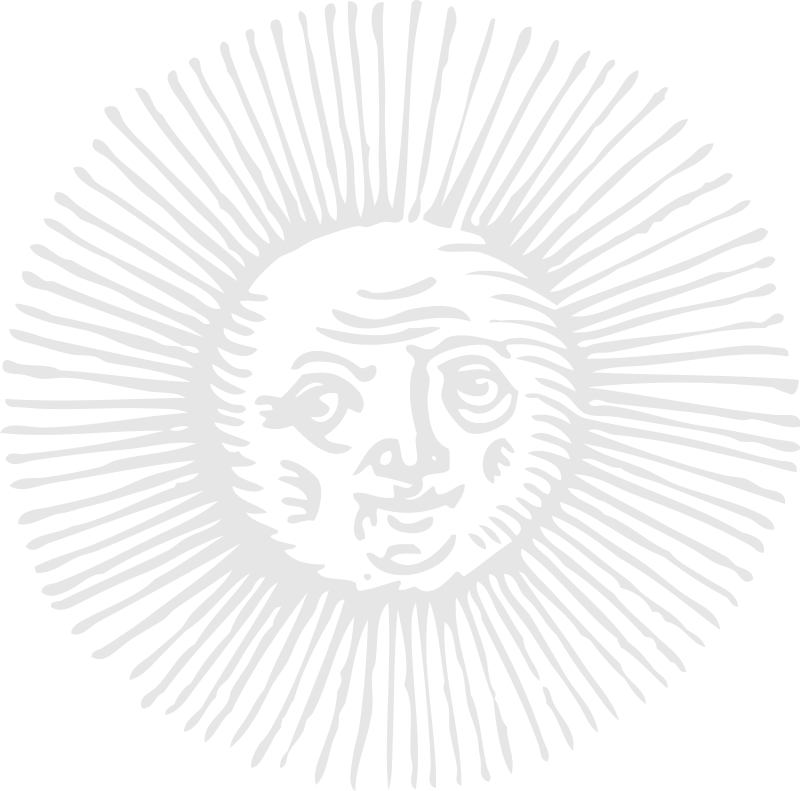
\includegraphics[scale=0.5]{../figs/johnny_automatic_old_sun_light}%
%\vfill
}}}


\author{Oscar Perpiñán Lamigueiro}
\date{\today}
\title{Preguntas breves}
\hypersetup{
 pdfauthor={Oscar Perpiñán Lamigueiro},
 pdftitle={Preguntas breves},
 pdfkeywords={},
 pdfsubject={},
 pdfcreator={Emacs 25.2.2 (Org mode 9.1.4)}, 
 pdflang={English}}
\begin{document}

\maketitle

\section*{Radiación Solar}
\label{sec:orgd76b38f}
\begin{itemize}
\item En las siguientes afirmaciones se resalta en negrita un
número. Indique y razone brevemente si esa cantidad resaltada es
factible en el contexto de la frase correspondiente.

\begin{itemize}
\item En un lugar con latitud 40ºN, el valor medio de la irradiación
extra-atmosférica diaria en Junio es de
\SI{11.6}{\kWh\per\meter\squared}. La media de los valores de
radiación global diaria registrados durante ese mes en una
estación meteorológica cercana es de \textbf{25.2 MJ/m\(^{\text{2}}\)}.
\end{itemize}

\item Se sitúa un módulo fotovoltaico orientado hacia el sur e inclinado
un ángulo igual a la latitud en un lugar del hemisferio norte con
latitud mayor que cero. Responda si son verdaderas o falsas las
siguientes afirmaciones, aportando una breve justificación de la
respuesta.
\begin{itemize}
\item En el instante del mediodía solar, en los solsticios, el coseno
del ángulo de incidencia entre el vector sol-tierra y la normal al
plano del módulo coincide con el del ángulo que forma el plano de
la eclíptica con el plano ecuatorial.
\end{itemize}
\end{itemize}

\begin{itemize}
\item En el instante del amanecer, el día del solsticio de invierno, el sol está situado detrás del módulo.
\end{itemize}

\begin{itemize}
\item Si utilizamos el modelo isotrópico para calcular la radiación
difusa, podemos afirmar que la cantidad de radiación difusa
captada por este módulo es siempre inferior a la captada por un
plano horizontal.
\end{itemize}

\begin{itemize}
\item El índice de claridad, \(K_{T}\), y la fracción de difusa, \(F_{D}\),
son dos parámetros que caracterizan el estado atmosférico en lo que
a radiación solar se refiere. En relación con estos dos parámetros,
responda si son verdaderas o falsas las siguientes afirmaciones,
aportando una breve justificación de la respuesta.

\begin{itemize}
\item La utilización de modelos anisotrópicos para estimar la radiación
difusa sobre una superficie inclinada es particularmente importante
cuando el valor de \(K_{T}\) es elevado.

\item \(K_{T}\) se define, en un determinado intervalo de tiempo, como la
relación entre la radiación global y la radiación directa, ambas
sobre superficie horizontal.

\item Suponga que, para un cierto periodo de tiempo, la relación entre
\(K_{T}\) y \(K_{D}\) puede representarse mediante la ecuación
\(K_{D}=b-a\cdot K_{T}\).
\begin{itemize}
\item El valor del coeficiente \(b\) es siempre mayor que 1.
\item El coeficiente a es siempre positivo.
\end{itemize}
\end{itemize}

\item Un determinado mes de un punto del hemisferio Norte se caracteriza
por un promedio mensual de irradiación global diaria en el plano
horizontal de \(\SI{5}{\kWh\per\meter\squared}\). El calculo del
promedio mensual de irradiación diaria extraterrestre en el plano
horizontal proporciona un valor de
\(\SI{7}{\kWh\per\meter\squared}\). Obtenga el valor del
correspondiente promedio mensual de irradiación difusa diaria en el
plano horizontal. Exprese los cálculos y resultados con nomenclatura
y unidades adecuadas. A la luz de estos valores, ¿a qué época del
año corresponde este mes?
\end{itemize}

\begin{itemize}
\item Necesita calcular el coseno del ángulo de incidencia sobre un
generador fotovoltaico estático. Dispone de la siguiente
información: día del año, hora oficial, latitud y longitud del
lugar. ¿Qué información adicional necesita conocer para realizar el
cálculo? Describa de forma concisa el procedimiento a seguir
contando con la información completa.
\end{itemize}

\begin{itemize}
\item Una estación meteorológica situada en el centro de la península
dispone de sensores de radiación solar que almacena en valores
diarios. Del análisis de esta información se estima que la media de
la irradiación global anual en el plano horizontal es de
\(\SI{6460}{\kWh\per\meter\squared}\). ¿Es aceptable este
valor? En caso contrario, expliqué por qué e indique un valor
orientativo que considere razonable. ¿Cuál puede ser el error
cometido al realizar la primera estimación?
\end{itemize}

\begin{itemize}
\item La inclinación óptima de un sistema fotovoltaico se calcula de forma
diferente teniendo en cuenta la aplicación del sistema. Indique la
ecuación correspondiente para las tres aplicaciones principales
(conexión a red, bombeo de agua, y electrificación rural)
\texttt{razonando} el motivo de cada una de estas ecuaciones.
\end{itemize}


\section*{Módulos y Generadores}
\label{sec:orge864506}
\begin{itemize}
\item En las siguientes afirmaciones se resalta en negrita un
número. Indique y razone brevemente si esa cantidad resaltada es
factible en el contexto de la frase correspondiente.
\begin{itemize}
\item Un módulo de silicio monocristalino con dimensiones 1000 x 800 mm
tiene una potencia de \textbf{275 Wp}.

\item Un módulo tiene 108 células de silicio monocristalino conectadas
en serie. Su tensión de circuito abierto en STC es de \textbf{24.2 V}.
\end{itemize}

\item En un momento determinado del día, un módulo de un seguidor a doble
eje está afectado por sombras arrojadas por otro
seguidor. Comparemos el funcionamiento de este módulo con otro
módulo perteneciente al mismo seguidor y no afectado por
sombras. Responda si son verdaderas o falsas las siguientes
afirmaciones, aportando una breve justificación de la respuesta.
\begin{itemize}
\item La corriente de cortocircuito del módulo sombreado es inferior a la
del módulo no sombreado.

\item La tensión de circuito abierto del módulo sombreado es inferior a la del módulo no sombreado.
\item La resistencia serie del módulo sombreado es inferior a la del módulo no sombreado.
\item La corriente en el punto de máxima potencia del módulo sombreado disminuye de forma proporcional a la radiación sombreada.
\item La disminución de radiación incidente debida al sombreado conlleva
una reducción en la temperatura del módulo sombreado. Por tanto, la
tensión en el punto de máxima potencia del módulo sombreado aumenta
a razón de \(2.3\,mV/^{\circ}C/celula\) con la diferencia entre la
temperatura de trabajo y la correspondiente a condiciones estándar
de test (STC).
\end{itemize}

\item Comente la validez de esta afirmación: ``El uso de diodos de paso
debe ser tenido en cuenta por el diseñador sólo cuando el generador
fotovoltaico vaya a estar sometido a condiciones de temperatura
ambiente especialmente elevadas. En caso contrario, se puede
prescindir del uso de estos elementos para reducir los costes del
sistema.''

\item Describa brevemente las causas y consecuencias del fenómeno del
punto caliente en los módulos fotovoltaicos. ¿Es razonable el uso de
varistores para evitar su aparición?
\end{itemize}

\begin{itemize}
\item En la fachada de un edificio existe un generador fotovoltaico. En un
momento determinado parte de este generador está afectado por
sombras de un arbolado cercano. Tomando en consideración dos módulos
de este generador, uno de ellos afectado por sombra y denominado
\(M_S\), y otro sin sombras y denominado \(M_0\), suponiendo que ambos
módulos son idénticos, compare las siguientes magnitudes usando
afirmaciones del estilo ``La [magnitud] del módulo \(M_s\) es mayor
que la del módulo \(M_0\) porque \ldots{}'':
\begin{itemize}
\item Corriente de cortocircuito
\item Tensión de circuito abierto
\item Temperatura de célula
\item Potencia eléctrica
\end{itemize}
\end{itemize}


\section*{SFCR}
\label{sec:orgdceeeec}
\begin{itemize}
\item En las siguientes afirmaciones se resalta en negrita un
número. Indique y razone brevemente si esa cantidad resaltada es
factible en el contexto de la frase correspondiente.

\begin{enumerate}
\item La media anual de la productividad diaria de un SFCR estático en
Madrid es de \textbf{6.5 kWh/kWp}.

\item Un generador FV está situado a 100 m de distancia de su
inversor. La tensión y corriente de trabajo en el tramo de
continua son 400 V y 10 A, respectivamente. Es necesario utilizar
una sección de cable de \textbf{35mm\(^{\text{2}}\)}.
\end{enumerate}

\item En relación con un inversor DC/AC, responda si son verdaderas o
falsas las siguientes afirmaciones, aportando una breve
justificación de la respuesta.

\begin{itemize}
\item Se emplea principalmente la tecnología de conmutación de onda
cuadrada, dada la sencillez de la lógica de control, el bajo nivel
de armónicos y la facilidad para regular el nivel de tensión de
salida.
\item Se suele elegir una frecuencia de conmutación superior a 1 MHz,
dada la baja influencia de la frecuencia en la distorsión de onda
y la relación inversamente proporcional entre la frecuencia y las
pérdidas por conmutación.
\item Para inversores de potencia inferior a 5 kW se emplea tecnología
de modulación del ancho de pulso mediante comparación con onda
sinusoidal (SPWM). Para potencias superiores, y dadas las
limitaciones de los dispositivos de conmutación, se utiliza
conmutación por onda cuadrada.
\end{itemize}

\item Un informe sobre una instalación fotovoltaica de conexión a red
proyectada en el sur de la península declara una media anual de la
productividad diaria de
\(\SI{4.1}{\kWh\per\kilo\Wp}\). Sabiendo que la
irradiación global efectiva anual en el plano del generador
correspondiente a esa localidad es de
\(\SI{1860}{\kWh\per\meter\squared}\), ¿cuál es el
\emph{performance ratio} de la instalación propuesta? Suponga que el
efecto de las sombras es despreciable.

\item Como es conocido, en los generadores fotovoltaicos de los SFCR se
recomienda la configuración flotante. Responda si son verdaderas o
falsas las siguientes afirmaciones, aportando una breve
justificación de la respuesta.

\begin{itemize}
\item De esta forma, se garantiza la prevención contra cortocircuitos y
sobrecargas debidas a la red eléctrica.

\item Así, se garantiza mayor protección tanto frente a contactos directos
como frente a contactos indirectos. Sin embargo, la protección
aumenta con una red de tierras bien diseñada y un vigilante de
aislamiento integrado en el inversor.

\item Esta configuración consiste en que todas las partes metálicas
accesibles son puestas a tierra junto con al menos un conductor
activo en la parte DC. Todos los conductores activos de la parte AC
quedan aislados de tierra.
\end{itemize}

\item Los equipos denominados inversores se emplean en los sistemas
autónomos de electrificación, en los sistemas de bombeo y en los
sistemas de conexión a red para convertir la corriente continua del
generador FV en corriente alterna. Indique las principales
diferencias que existen entre los inversores adecuados a cada una de
estas tres aplicaciones.
\end{itemize}
\end{document}